% This is the Reed College LaTeX thesis template. Most of the work 
% for the document class was done by Sam Noble (SN), as well as this
% template. Later comments etc. by Ben Salzberg (BTS). Additional
% restructuring and APA support by Jess Youngberg (JY).
% Your comments and suggestions are more than welcome; please email
% them to cus@reed.edu
%
% See http://web.reed.edu/cis/help/latex.html for help. There are a 
% great bunch of help pages there, with notes on
% getting started, bibtex, etc. Go there and read it if you're not
% already familiar with LaTeX.
%
% Any line that starts with a percent symbol is a comment. 
% They won't show up in the document, and are useful for notes 
% to yourself and explaining commands. 
% Commenting also removes a line from the document; 
% very handy for troubleshooting problems. -BTS

% As far as I know, this follows the requirements laid out in 
% the 2002-2003 Senior Handbook. Ask a librarian to check the 
% document before binding. -SN

%%
%% Preamble
%%
% \documentclass{<something>} must begin each LaTeX document
\documentclass[12pt,twoside]{reedthesis}
% Packages are extensions to the basic LaTeX functions. Whatever you
% want to typeset, there is probably a package out there for it.
% Chemistry (chemtex), screenplays, you name it.
% Check out CTAN to see: http://www.ctan.org/
%%
\usepackage{graphicx,latexsym} 
\usepackage{amssymb,amsthm,amsmath}
\usepackage{longtable,booktabs,setspace} 
\usepackage{chemarr} %% Useful for one reaction arrow, useless if you're not a chem major
\usepackage[hyphens]{url}
\usepackage{rotating}
\usepackage{natbib}
\usepackage{color}
\graphicspath{{./Figs/}} % Set graphics path
% Comment out the natbib line above and uncomment the following two lines to use the new 
% biblatex-chicago style, for Chicago A. Also make some changes at the end where the 
% bibliography is included. 
%\usepackage{biblatex-chicago}
%\bibliography{thesis}

% \usepackage{times} % other fonts are available like times, bookman, charter, palatino


%%%% REFERENCES %%%%%
\newcommand{\rf}     [1] {~\cite{#1}}
\newif\ifimagesSep
\newcommand*{\rfs}[1]{%
  \par\noindent[begin images]\\\relax
  \imagesSepfalse
  \imagesScan#1\relax\relax\relax
  [end images]\par
}
\newcommand{\imagesScan}[3]{%
  \ifx\relax#1\empty
  \else
    \ifimagesSep
      [separation]\\\relax
    \else
      \imagesSeptrue
    \fi
    [image: #1 #2 #3]\\\relax
    \expandafter\imagesScan
  \fi
}

\newcommand{\refref} [1] {ref.~\cite{#1}}
\newcommand{\refRef} [1] {Ref.~\cite{#1}}
\newcommand{\refrefs}[1] {refs.~\cite{#1}}
\newcommand{\refRefs}[1] {Refs.~\cite{#1}}
\newcommand{\refeq}  [1] {(\ref{#1})}
\newcommand{\refeqs} [2]{(\ref{#1}--\ref{#2})}
\newcommand{\reffig} [1] {figure~\ref{#1}}
\newcommand{\reffigs} [2] {figures~\ref{#1} and~\ref{#2}}
\newcommand{\refFig} [1] {Figure~\ref{#1}}
\newcommand{\refFigs} [2] {Figures~\ref{#1} and~\ref{#2}}
\newcommand{\reftab} [1] {table~\ref{#1}}
\newcommand{\refTab} [1] {Table~\ref{#1}}
\newcommand{\reftabs}[2] {tables~\ref{#1} and~\ref{#2}}
\newcommand{\refsect}[1] {Section~\ref{#1}}
\newcommand{\refsects}[2] {Sections~\ref{#1} and \ref{#2}}
\newcommand{\refSect}[1] {Sect.~\ref{#1}}
\newcommand{\refSects}[2] {Sects.~\ref{#1} and \ref{#2}}
\newcommand{\refsecttosect}[2] {Sects.~\ref{#1} to~\ref{#2}}
\newcommand{\refappe}[1] {appendix~\ref{#1}}
\newcommand{\refappes}[2] {appendices~\ref{#1} and~\ref{#2}}
\newcommand{\refAppe}[1] {Appendix~\ref{#1}}
\newcommand{\refChapter}[1]{Chapter~\ref{#1}}
\newcommand{\refChapt}[1]{Chapt.~\ref{#1}}

%%%% SYMBOLS %%%%
\newcommand{\ReN}{\ensuremath{Re}} % Reynolds number
\newcommand{\pCf}{plane Couette flow} % plane Couette flow
\newcommand{\ecs}{exact coherent structures}
\newcommand{\Ecs}{Exact coherent structures}
%%%% ABBREVIATIONS %%%%%
\newcommand{\etc}{{etc.}}       % APS
\newcommand{\etal}{{\em et al.}}    % etal in italics, APS too
\newcommand{\ie}{{i.e.}}        % APS
\newcommand{\cf}{{\em cf.\ }}     % APS
\newcommand{\eg}{{e.g.\ }}        % APS, OUP, hard space '\eg\ NextWord'

%%%%% EDITING COMMANDS %%%%%
\newcommand{\DB}[2]{$\footnotemark\footnotetext{DB #1: {\color{red}#2}}$} %date, comment
\newcommand{\DBedit}[1]{{\color{red}#1}}
\newcommand{\VGC}[2]{$\footnotemark\footnotetext{DB #1: {\color{blue}#2}}$} %date, comment
\newcommand{\VGedit}[1]{{\color{blue}#1}}


%%%% SUPER USEFUL COMMANDS THAT I'M USED TO HAVING%%%%%
\let\Oldfrac\frac
\renewcommand{\frac}[2]{\dfrac{#1}{#2}}

\let\Oldsin\sin
\renewcommand{\sin}[1]{\Oldsin{\left ( #1  \right ) }}

\let\Oldcos\cos
\renewcommand{\cos}[1]{\Oldcos{\left ( #1  \right ) }}

\newcommand{\abs}[1]{\left | #1 \right |}
\newcommand{\sqfrac}[2]{\sqrt{\frac{#1}{#2}}}
\newcommand{\paren}[1]{\left ( #1 \right )}
\newcommand{\sbrac}[1]{\left [ #1 \right ]}
\newcommand{\scprod}[3]{\left < #1,#2 \right >_{#3}}

\let\Oldint\int
\renewcommand{\int}[4]{\Oldint_{#1}^{#2} #3 \hspace{2mm}#4}
\let\Oldsum\sum
\renewcommand{\sum}[3]{\Oldsum\limits_{#1}^{#2} #3}


\newcommand{\pder}[3]{\ifnum#1=1
							\dfrac{\partial#2}{\partial#3}
					   \else
					   \ifnum#1>1\dfrac{\partial^{#1}#2}{\partial#3^{#1}} \fi \fi }
\newcommand{\der}[3]{\ifnum#1=1
							\dfrac{\text{d}#2}{\text{d}#3}
					   \else
					   \ifnum#1>1\dfrac{\text{d}^{#1}#2}{\text{d}#3^{#1}} \fi \fi }
\newcommand{\Vector}[1]{\mathbf{#1}}
\newcommand{\Tensor}[1]{\mathcal{#1}}
\newcommand{\function}[2]{#1\!\paren{#2}}

\newcommand{\Div}[1]{\nabla\cdot#1}
\newcommand{\Grad}[1]{\nabla\,#1}
\newcommand{\equationref}[1]{Equation~\ref{#1}}
\newcommand{\figureref}[1]{Figure~\ref{#1}} % Load thesis specific macros

\title{My Final College Paper}
\author{Your R. Name}
% The month and year that you submit your FINAL draft TO THE LIBRARY (May or December)
\date{May 200x}
\division{Mathematics and Natural Sciences}
\advisor{Advisor F. Name}
%If you have two advisors for some reason, you can use the following
%\altadvisor{Your Other Advisor}
%%% Remember to use the correct department!
\department{Mathematics}
% if you're writing a thesis in an interdisciplinary major,
% uncomment the line below and change the text as appropriate.
% check the Senior Handbook if unsure.
%\thedivisionof{The Established Interdisciplinary Committee for}
% if you want the approval page to say "Approved for the Committee",
% uncomment the next line
%\approvedforthe{Committee}

\setlength{\parskip}{0pt}
%%
%% End Preamble
%%
%% The fun begins:
\begin{document}

  \maketitle
  \frontmatter % this stuff will be roman-numbered
  \pagestyle{empty} % this removes page numbers from the frontmatter

% Acknowledgements (Acceptable American spelling) are optional
% So are Acknowledgments (proper English spelling)
%	% Acknowledgements (Acceptable American spelling) are optional
% So are Acknowledgments (proper English spelling)
    \chapter*{Acknowledgments}
	\epigraph{Some people are of the opinion that acknowledgments ought to be concise, relevant to the thesis, and devoid of sappy sentiment. They are probably right, but they aren't the ones writing this.}{Varchas Gopalaswamy}

This thesis wouldn't have existed without my thesis advisor, Daniel Borrero. Thank you, Daniel, for suggesting an awesome thesis topic, for motivating me, for spending a ton of time correcting more terrible thesis drafts than any human should have to, for introducing me to dynamical systems theory, and for all the grad school help. Good luck with setting up the Taylor-Couette system.\\

I would also like to thank John Gibson from the University of New Hampshire for making this thesis even remotely feasible by writing {\tt Channelflow}, and for taking the time to correspond with me via email and Hangout. Your advice has been invaluable. \\
 
By definition, this thesis wouldn't have existed were I not a physics major, so I'd like to thank the department as a whole for being the greatest department at Reed. Thank you, Lucas, for being an extremely supportive academic advisor and for a  challenging junior year. Thank you, Joel, for introducing me to the world of scientific computation, for running physics softball, and for your help with this thesis. Thank you, Darrell, for reminding me why quantum mechanics is awesome. Thank you, Johnny, for all the help with the grad school process. Thanks also to the physics seniors -- shoutout to Julia and Neal for their tenure as the Pub Czars, Taras for his tenure as the Cookie Czar, Dan for putting up with the frantic late night calls for help, and Newton for being a rad office buddy.  I will be proud to say that I was once a part of this group. You guys have made my time here special. \\

To Amma and Appa -- Thank you for all your love and support throughout all these years, and always being understanding and there for me when I have the occasional mental breakdown. Also, thanks for going ``Yes, let's send Varchas to this college we've literally never heard anything about, this sounds like a great idea." I hope you feel that you've made the right decision. 

Dear Medha: Thank you for allowing me to lecture at you about stuff you may or may not actually be interested in, for enabling me in some truly horrendous jokes, for doing all the housework whenever I would come back for vacation, and generally being an awesome sister. \\

To all my friends -- Thank you for making Reed the best of times, and for supporting me through the worst of times. Words cannot express how much I will miss you all.\footnote{Yes Matt, even you.}






% The preface is optional
% To remove it, comment it out or delete it.
%	% The preface is optional
% To remove it, comment it out or delete it.
    \chapter*{Preface}
	This is an example of a thesis setup to use the reed thesis document class.

%  \tableofcontents
% if you want a list of tables, optional
%  \listoftables
% if you want a list of figures, also optional
%  \listoffigures
		
% The abstract is not required if you're writing a creative thesis (but aren't they all?)
% If your abstract is longer than a page, there may be a formatting issue.
	%% The abstract is not required if you're writing a creative thesis (but aren't they all?)
% If your abstract is longer than a page, there may be a formatting issue.
    \chapter*{Abstract}
	\Ecs are an exciting and potentially revolutionary method of understanding turbulent dynamics and transition. In \pCf, the inherent symmetries naturally lead to symmetric \ecs, which are computationally easier to find. However, turbulence itself is a fundamentally asymmetric phenomenon, and may be better described by symmetry broken \ecs. In this thesis, we find four new periodic orbits -- P85 and P60m which have unbroken symmetry and P32 and P8, which have partially broken symmetry, using the computational fluid dynamics library {\tt Channelflow}. Comparison of the projections of these periodic orbits in the dissipation-energy input plane with randomly seeded turbulent trajectories reveals that P32, P60 and P85 lie in the turbulent region, while P8 lies very far away from the turbulent region. Nevertheless, we focus on P8 so as to best utilize limited computational resources. Parametric continuation in the spanwise periodic cell length $L_z$ suggests that P8 undergoes two bifurcations. This is verified by analysis of various properties of P8 in the dissipation-energy input plane, as well as an observation of a change of stability of eigenvectors that are consistent with the bifurcation.   
	%	\chapter*{Dedication}
	To Perfect Woodbridge \\
	\emph{sic transit gloria mundi}

  \mainmatter % here the regular arabic numbering starts
  \pagestyle{fancyplain} % turns page numbering back on

% Double spacing: if you want to double space, or one and a half 
% space, uncomment one of the following lines. You can go back to 
% single spacing with the \singlespacing command.
% \onehalfspacing
% \doublespacing

	%%The \introduction command is provided as a convenience.
%if you want special chapter formatting, you'll probably want to avoid using it altogether
		\setcounter{secnumdepth}{0}
\chapter*{Introduction}
    \addcontentsline{toc}{chapter}{Introduction}
		\chaptermark{Introduction}
		\markboth{Introduction}{Introduction}

% The three lines above are to make sure that the headers are right, that the intro gets included in the table of contents, and that it doesn't get numbered 1 so that chapter one is 1.
\epigraph{ I am an old man now, and when I die and go to heaven, there are two matters on which I hope for enlightenment. One is quantum electrodynamics, and the other is the turbulent motion of fluids. And about the former, I am optimistic. }{Horace Lamb, 1932}
	
Although much work has been done in understanding turbulence since Lamb's time, the twin problems of understanding the nature of the transition to turbulence and predicting the fine structure of turbulent flows remain unsolved to this day, having vexed scientists and engineers in much the same way a plucky band of Gauls did for Caesar. Understanding turbulence is vitally important, since turbulent flows appear in man-made scenarios such as the flow around ships or aircraft, as well as in natural scenarios like the atmosphere of Jupiter and the flow of blood in the heart. The degree to which a flow is turbulent is characterized by its {\bf Reynolds number} \ReN, a dimensionless parameter that encodes the relative importance of inertial and viscous forces. At small \ReN, the {\bf viscosity} of a fluid (which is analogous to fluid friction) dominates, and smooths out velocity gradients in the flow, resulting in well-ordered, {\bf laminar} flow. At large \ReN, kinetic energy is dissipated at a lower rate, allowing for the existence of increasingly complex flow structures such as eddies or vortices (\refFig{fig:cylinderWake}). These structures, which are typical of {\bf turbulence}, display large spatiotemporal variations and structure at a variety of spatial and temporal scales.
\begin{figure}[h]
\centerline{
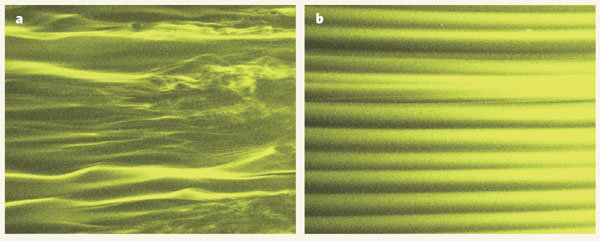
\includegraphics[width=\textwidth]{Figs/laminarTurbulent}}
\caption[Streamlines on two surfaces of differing smoothness showcase the difference between laminar and turbulent flows.]{Streamlines on two surfaces of differing smoothness showcase the difference between laminar and turbulent flows. (a) In turbulent flow across an extremely smooth surface, streamlines break up into chaotic eddies and swirls, while in (b), the laminar flow across a rough surface preserves the streamlines. Reproduced from K.S. Choi, ``Fluid Dynamics: The rough with the smooth", \emph{Nature},  vol. 440, no, 7085, pp. 754-754, 2006\rf{Choi2006}.}\label{fig:cylinderWake}
\end{figure}
\begin{figure}[h!]
\centerline{
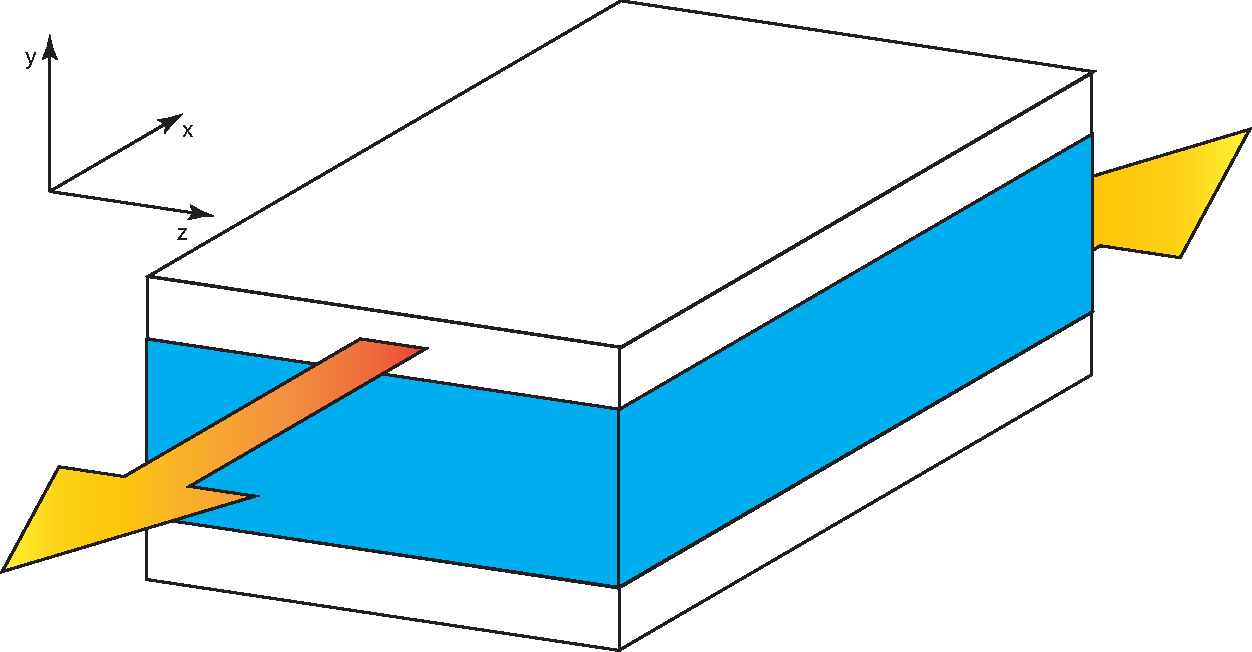
\includegraphics[scale=0.4]{Figs/planeCouetteDiagram}}
\caption[A schematic of the plane Couette geometry.]{A schematic of the plane Couette geometry. The upper and lower plates (white) extend infinitely in the plane, as does the fluid (blue) filling the gap between them. The upper and lower plates move with some constant velocity, and apply shear stresses to the fluid, resulting in fluid motion. While in general the plates can move in any direction, there is always a reference frame in which the plates move with equal but opposite velocity and it is convenient to work in this reference frame. According to convention, the $x$ axis is aligned along the plate velocity and is referred to as the {\bf streamwise} direction. The $y$-axis is aligned perpendicular to the plates and is referred to as the {\bf wall-normal} direction. The $z$-axis is normal to both axes and is referred to as the {\bf spanwise} direction.}\label{fig:planeCouette}
\end{figure}

\section{Plane Couette Flow} 

Since viscosity is a dissipative force, a viscous fluid that has no energy input will eventually come to rest as its kinetic energy is dissipated into thermal energy. Therefore, sustaining turbulence requires continuous energy input. In the case of the flow between two infinite parallel plates (\refFig{fig:planeCouette}), which is known as \pCf\ and is the focus of this thesis, this is provided by the wall shear. The geometry of the plane Couette system is extremely simple, with a geometrical parameter $h$, the half-distance between the parallel plates, and a kinematic parameter $V$, the constant velocity of the upper plate. This gives the Reynolds number as 
\begin{equation}
\ReN = \frac{hV}{\nu},
\end{equation}
where $\nu$ is the kinematic viscosity of the fluid. When \ReN~is very small, only the laminar flow state is stable. In the case of \pCf\ this corresponds to a linear velocity profile, shown in \refFig{fig:planeCouetteBulk}. As \ReN~increases, experiments\rf{Daviaud1992} have demonstrated the existence of long-lived turbulent flows, despite the fact that linear stability analysis predicts that the laminar state should remain stable.
\begin{figure}
\centerline{
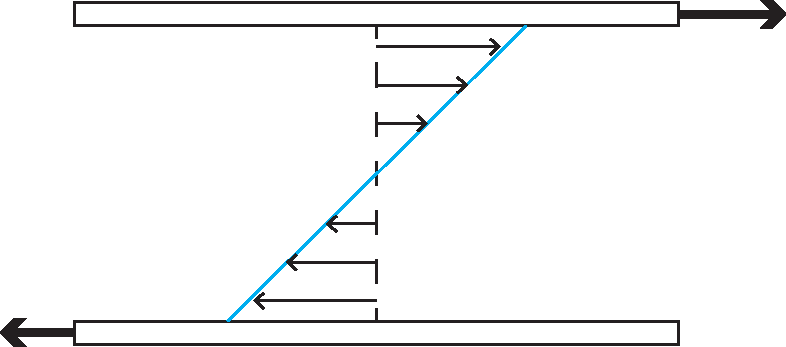
\includegraphics[scale=0.6]{Figs/planeCouetteMeanFlow}}
\caption[A cross-sectional representation of \pCf, with the linear, laminar velocity profile shown.]{A cross-sectional representation of \pCf, with the linear, laminar velocity profile shown. By symmetry, the laminar profile must be the same everywhere. At the top and bottom, where the fluid meets the walls, no-slip boundary conditions require that the wall-tangent velocity equal the boundary velocity.}\label{fig:planeCouetteBulk}
\end{figure}

\section{Tackling Turbulence} 

The traditional approach for the analysis of turbulent flow is the statistical approach initially developed by Reynolds, Prandtl, von Karman, Kolmogorov and others\rf{Pope2000}. At the core of the statistical approach to turbulence is the assumption that turbulent flow states can be expressed as random perturbations around some mean flow. At high \ReN, where direct numerical simulation (DNS) of the flow is computationally infeasible,\footnote{In essence, this is due to the fact that the minimum computational resolution required for DNS scales as $\ReN^{2.25}$ in 3D. As a result, the numerical resolution required to resolve even moderate \ReN\ flows is huge.}  the statistical approach is invaluable. However, at low-to-moderate \ReN, these models can become less accurate\rf{Pope2000}. Even ignoring the moderate \ReN\ behavior of the statistical models, a fundamental problem with the statistical approach is that it discards much of the dynamical information about turbulence. Some statistical methods like Reynolds Averaged Navier-Stokes choose to time-average the Navier-Stokes equations, while others like Large Eddy Simulations model all small length scale behavior, resolving only large length scales. For this reason, it seems likely that while statistical methods will remain fundamental to applied computational fluid dynamics (CFD), especially in engineering practice, they cannot truly provide an answer to the turbulence problem. \\

An alternate approach was proposed by Eberhard Hopf in 1948\rf{Hopf1948}. Hopf suggested that solutions to the Navier-Stokes equations might be thought of as trajectories in an infinite dimensional state space in which each point corresponded to a possible velocity field. To better understand what this would mean, consider the mean velocity field of some infinitesimal volume of fluid, pictured in \refFig{fig:VectorSpace}. In order to describe the velocity at a point in the fluid, three numbers are required (each of which can take any real value), so this vector lives in a three dimensional vector space. Now any finite fluid volume will have an infinite number of points at which the velocity field has to be specified, so we would need an infinite set of numbers to describe the full velocity field. An object that would keep track of all these numbers would form an infinite dimensional vector $\Vector{v} = \{v_{i,1},v_{i,2},v_{i,3}...\},~i \in \mathbb{R}$, so that any flow state would be represented by a unique vector in this infinite dimensional vector space, which is known as the {\bf state space}. 


\begin{figure}
\centerline{
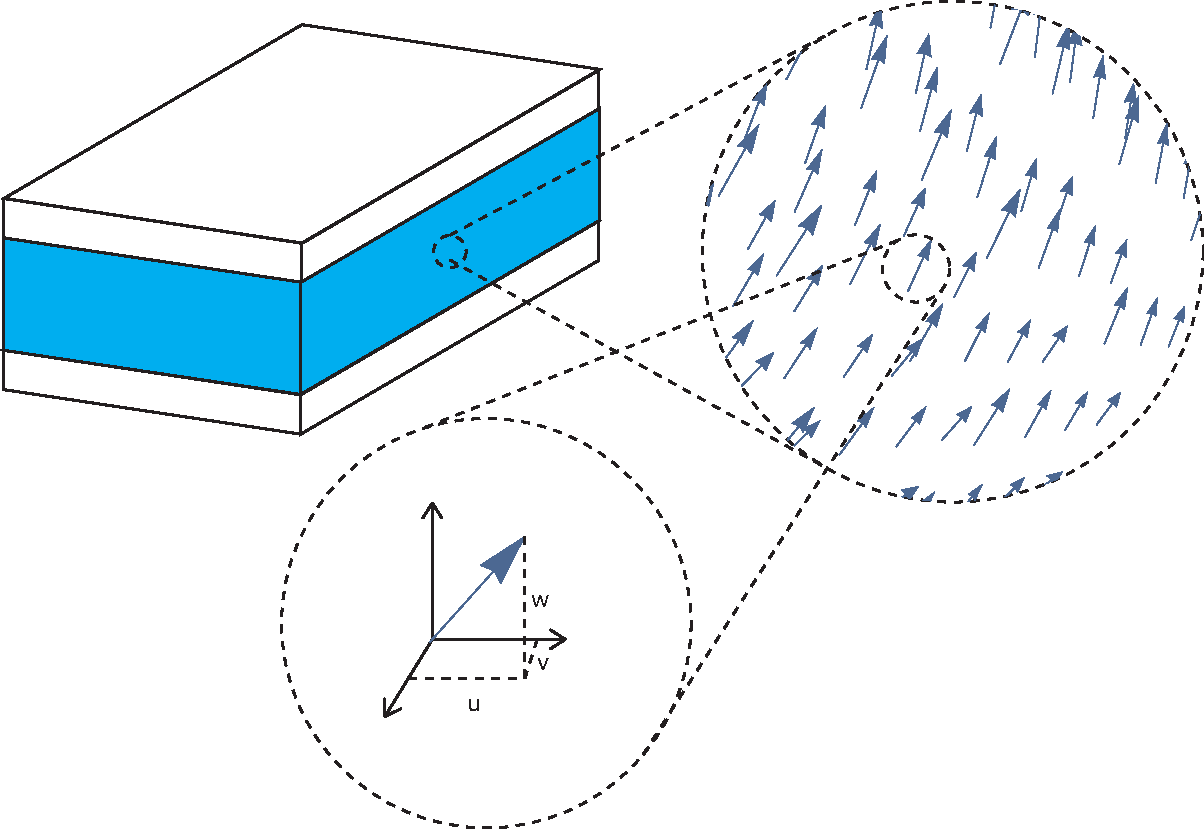
\includegraphics[scale=0.6]{Figs/VectorSpace}}
\caption{At each point in the fluid volume, the velocity field has a value that is described by three numbers, thus requiring three dimensions to track over time.}\label{fig:VectorSpace}
\end{figure}


Luckily, every point in the space does not necessarily correspond to a solution of the Navier-Stokes equation; for a given finite \ReN, for instance, the gradient of the velocity field cannot be too large since it would be smoothed out by viscosity. Hopf thus conjectured that physical trajectories corresponding to solutions to the Navier-Stokes equation would lie on some finite-dimensional manifold (known as the {\bf inertial manifold}) embedded within this infinite dimensional space. The restriction of dynamics from the infinite dimensional space to a finite dimensional inertial manifold due to the variation of a control parameter\footnote{The control parameter of a dynamical system is a number that is time-independent, and typically dictates the behavior of the system in some way. For instance, in the dimensionless simple harmonic oscillator, $\ddot{x} + 2\zeta \dot{x} + x = 0$, the control parameter is the dimensionless number $\zeta$, whose value determines whether the system is undamped, underdamped, over damped or critically damped.} has been rigorously proven under certain conditions\rf{Foias1988}. For the Navier-Stokes equation, the inertial manifold's control parameter is \ReN, and physical intuition suggests that its structure should also have \ReN~dependence, since at very low \ReN, the only physical solution is the laminar state which corresponds to a point in the state space. As \ReN\ increases, more complex flows become physically permissible, so the inertial manifold grows from a point of dimension 0 into a more complex, higher dimensional manifold. Hopf proposed that turbulence in this view was simply a trajectory that would travel across wide distances on the inertial manifold. \\


\begin{figure}[h]
\centerline{
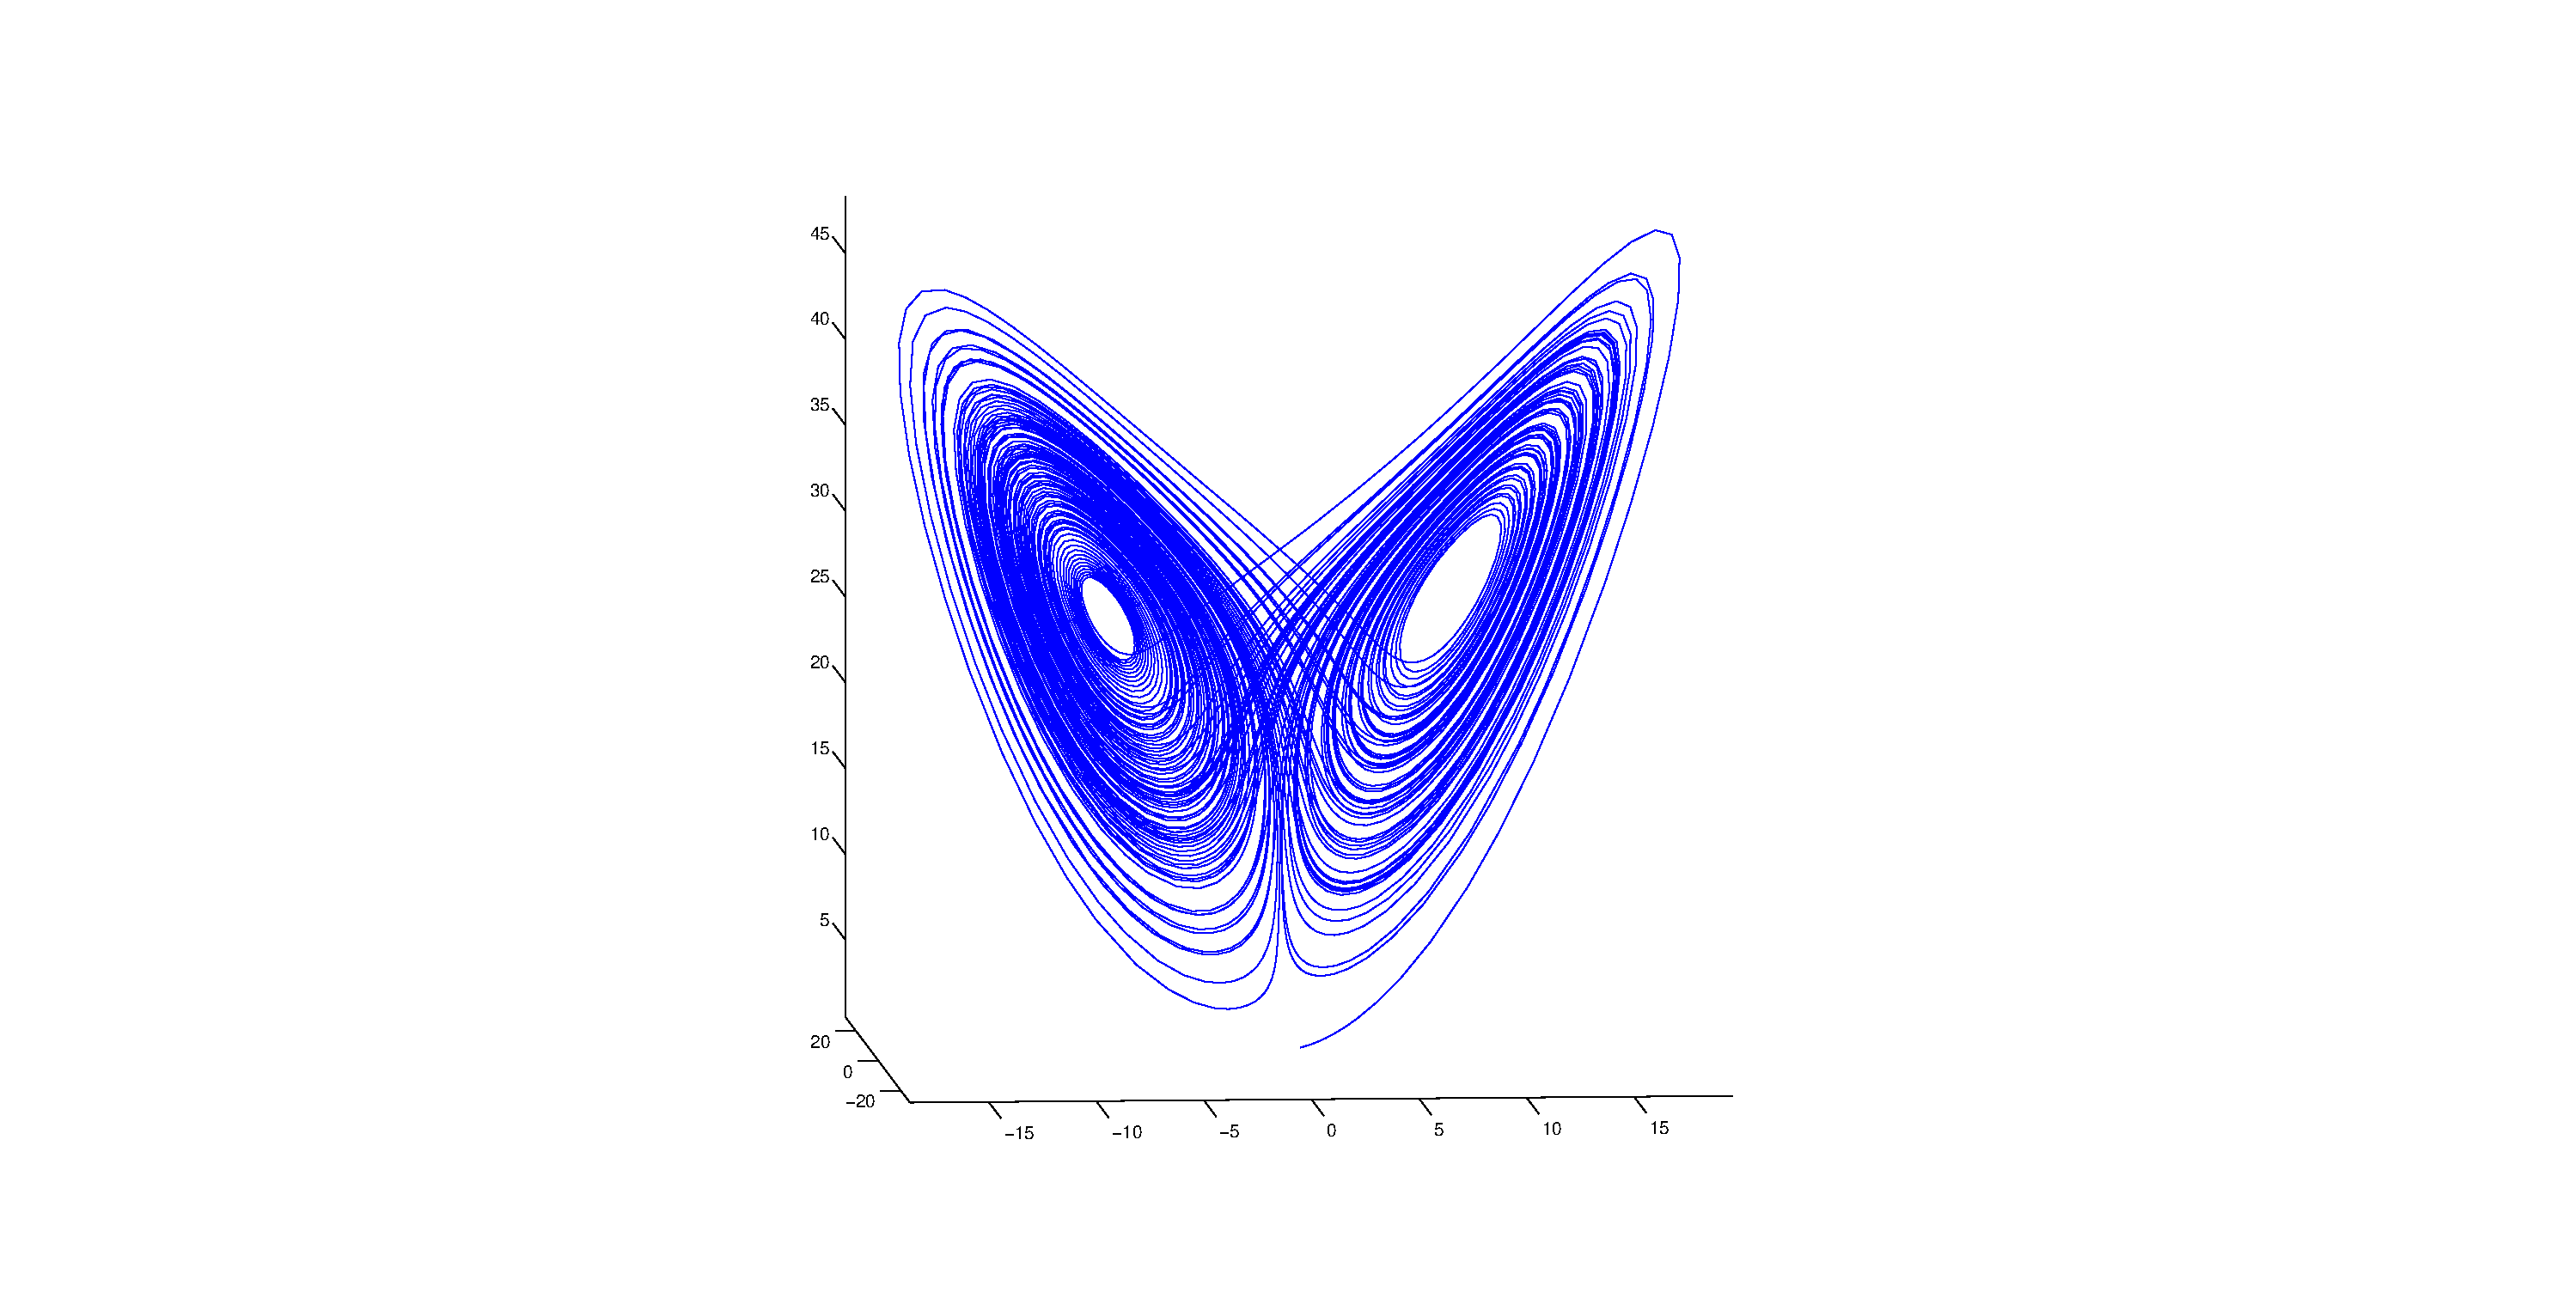
\includegraphics[scale=0.5	]{Figs/LorenzAttractor}}
\caption[A plot of a trajectory for the Lorenz system.]{A plot of a trajectory for the Lorenz system. The Lorenz system is an excellent example of a system in which the dynamics collapse onto an inertial manifold - in this case, the dynamics exist on a manifold of fractal dimension 2.06\rf{Grassberger2004}, even though the state space is in three dimensions. }\label{fig:LorenzAttractor}
\end{figure}

Unfortunately for Hopf, the computer power necessary to pursue this line of work was not available in 1948, leading him to comment in frustration that ``“the great mathematical difficulties of these important problems are well
known and at present the way to a successful attack on them seems hopelessly
barred"\rf{Hopf1948}. It would take until 1963 and the derivation of the Lorenz system (\refFig{fig:LorenzAttractor}) for the first numerical state-space analysis of turbulence\rf{Lorenz1963}, albeit for a highly truncated version of Navier-Stokes, designed to investigate Rayleigh-Bernard convection.\footnote{Interestingly, Lorenz truncated Navier-Stoke via a Galerkin approximation, which is what the simulation library {\tt Channelflow} which features heavily in this thesis also does, though it allows for many more Fourier modes than Lorenz did.} There have also been a number of efforts to explore the structure of invariant manifolds in moderate \ReN\ turbulence Navier-Stokes, such as Proper Orthogonal Decomposition\rf{Aubry1988} and the `self-sustaining process theory'\rf{Dauchot2000}, which while fruitful, are nevertheless models of turbulent flow, and not an exact analysis of the Navier-Stokes equations.\\


\begin{figure}[h]
\centerline{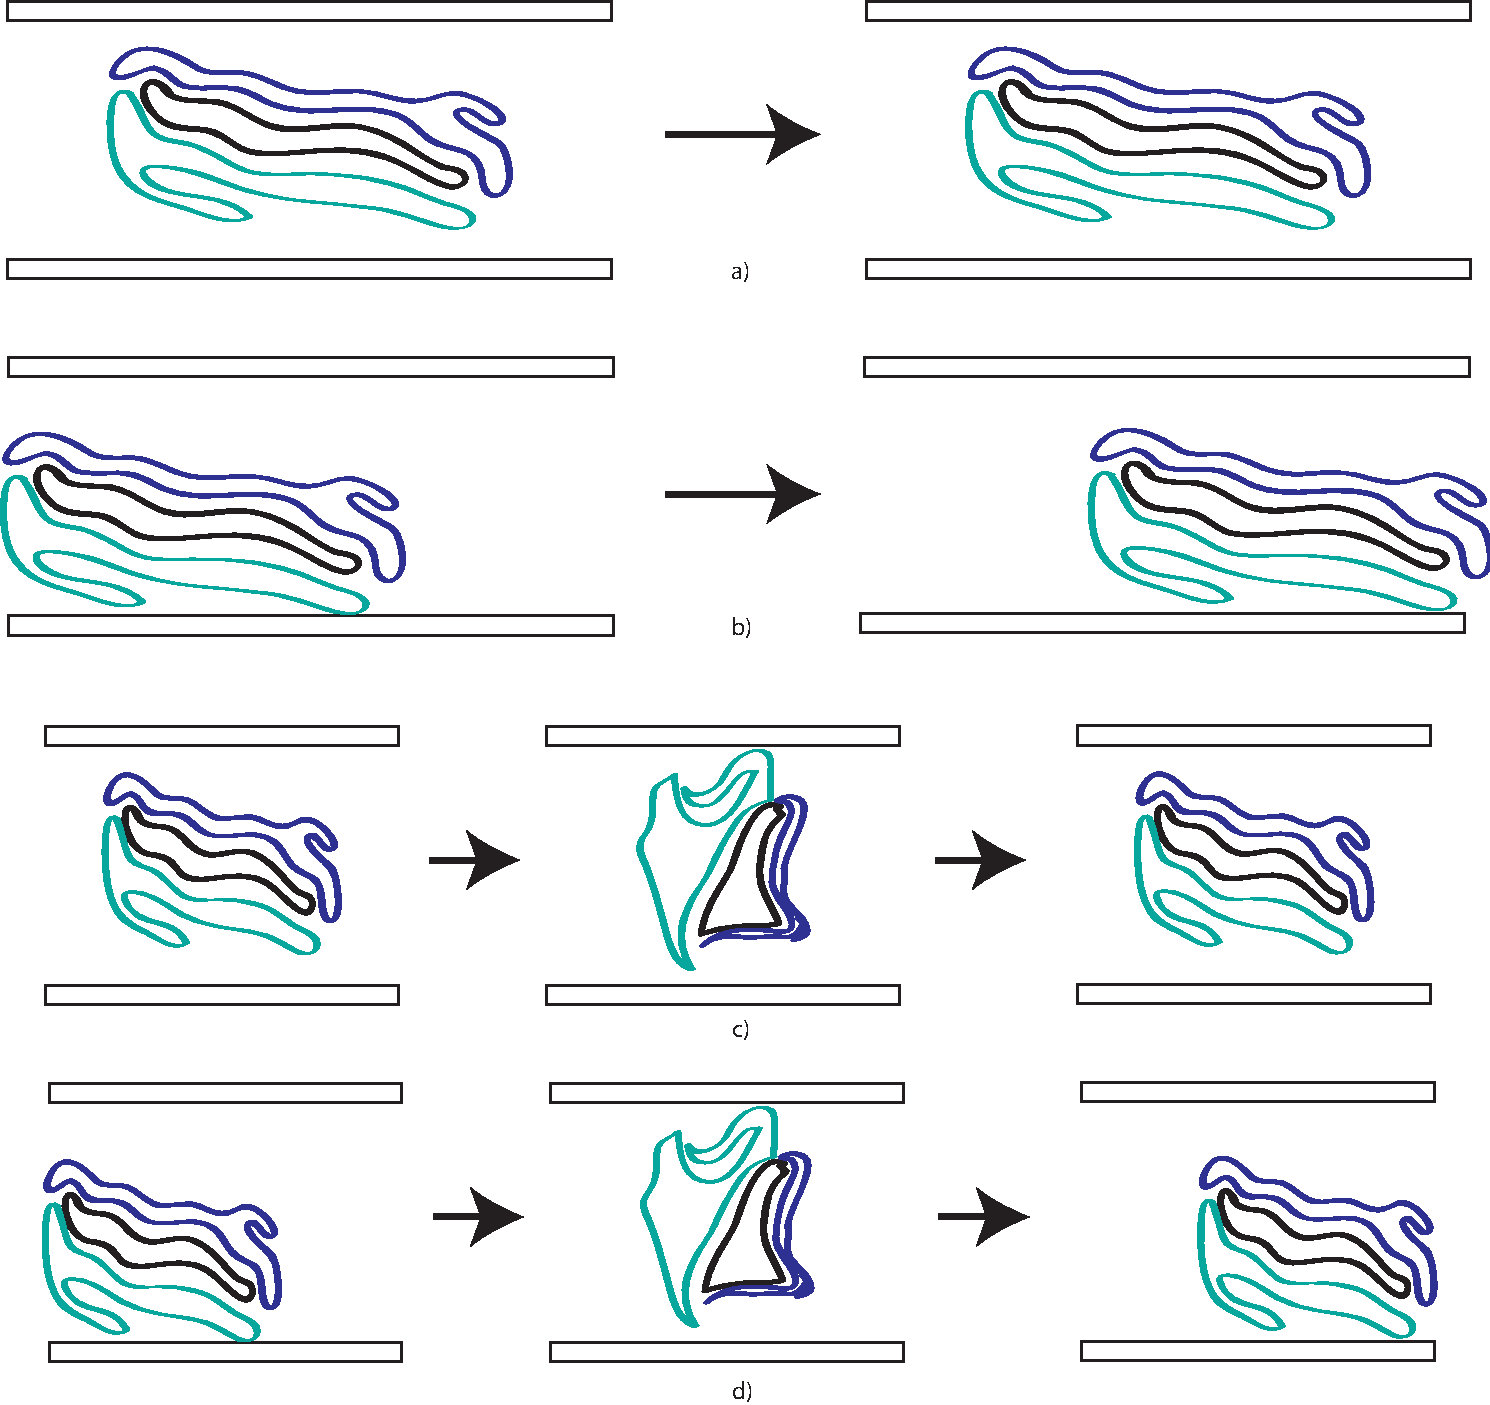
\includegraphics[scale=0.5]{Figs/ECSClassification}}
\caption[The four main categories of \ecs.]{The four main categories of \ecs. In all diagrams, only a particular flow structure is displayed, to demonstrate the various types of \ecs. These could be, for example, isosurfaces of velocity or energy. (a) An {equilibrium} solution, where the fluid structure does not change over time. (b) A {relative equilibrium} or {traveling wave} solution, where the state does not change in its own reference frame, but is translated relative to the observer. (c) A {periodic orbit}, where the flow state changes over time, but returns to the original state after some period $T$. (d) A {relative periodic orbit}, where the flow state is periodic in its own reference frame, but is translated relative to the observer.}\label{fig:ECS}
\end{figure}


Another avenue of research emerged in 1990, when Nagata computed nontrivial {\bf equilibrium} flow states for \pCf\ by continuing the wavy vortex solution of Taylor-Couette flow\rf{Nagata1990}. This class of solutions, which were named {\bf exact coherent structures} by Waleffe\rf{Waleffe2001} are the result of calculating exact, invariant solutions of the fully resolved Navier-Stokes equations. The family of \ecs\ was expanded with the discovery of {\bf traveling wave equilibria} by Nagata in 1997, the computation of {\bf periodic orbits} by Kawahara and Kida in 2001\rf{Kawahara2001}, and the computation of {\bf relative periodic orbits}\footnote{That is, flow states that are periodic after some phase shift.} by Viswanath in 2007\rf{Viswanath2007}. \refFig{fig:ECS} summarizes these four categories of \ecs. The ultimate hope of this line of research is that turbulence can be viewed as chaotic trajectories on the inertial manifold that are guided by hyperbolic \ecs\footnote{That is to say, the \ecs\ have many stable directions that are highly attractive and pull trajectories towards them, and a few unstable directions that ultimately eject the trajectory.} (\refFig{fig:guidedTurbulence}). \\

\begin{figure}[h]
\centerline{
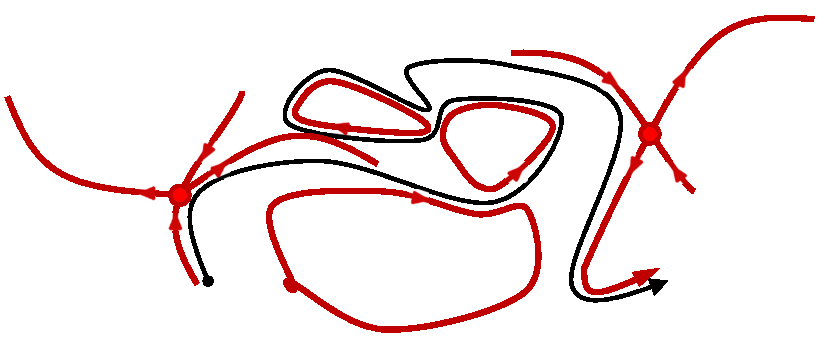
\includegraphics[width=\textwidth]{Figs/phaseSpaceTraj.pdf}}
\caption[A schematic of a turbulent trajectory in state space and the coherent structures that guide it.]{A schematic of a turbulent trajectory in state space and the coherent structures that guide it. (a) A turbulent trajectory in black appears chaotic and unpredictable in isolation. (b) When the underlying coherent structures in red are superimposed, however, the guiding of the dynamics by the \ecs\ becomes evident. Starting from the left, the trajectory is pulled in towards an equilibrium (filled circle) along its stable manifold (arrow pointing inwards), before being ejected along its unstable manifold (arrow pointing outwards). The trajectory then shadows three periodic orbits, whose stable and unstable manifolds are not trivial to represent visually, but nonetheless exist, before being attracted and ejected by the final equilibrium and continuing on its way. Reproduced from D. Borrero-Echeverry, \emph{Subcritical Transition to Turbulence in Taylor-Couette Flow}, PhD. Dissertation, Dept. of Physics, Georgia Institute of Technology, 2014\rf{Borrero2014}.}\label{fig:guidedTurbulence}
\end{figure}

\begin{figure}[t]
\centerline{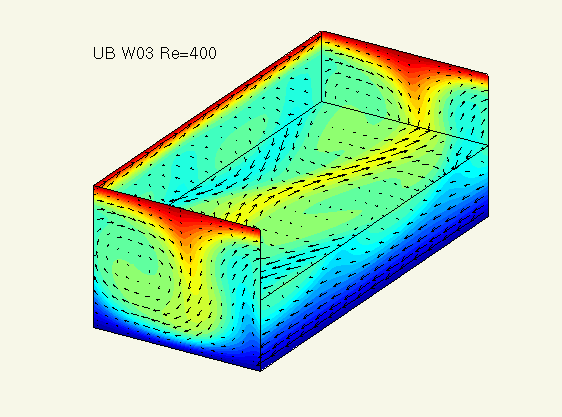
\includegraphics[scale=0.5]{Figs/rollStreak}}
\caption[The roll-streak structure of the Nagata upper branch equilibrium]{The roll-streak structure of the Nagata upper branch equilibrium\rf{Nagata1990}. The in-plane velocity vectors in the periodic cell are displayed for the box walls, as well as the mid-plane. The coloration reflects the streamwise velocity, where blue indicates a large streamwise velocity out of the page, and red represents a large streamwise velocity into the page. The vortex that forms the roll is clearly visible on the near box wall, as is the streak running through the midplane of the box. These structural features are often seen in real turbulent flows, and solutions that approach the vicinity of this solution in the state space will take on some of this roll-streak structure. Reproduced from J. F. Gibson, J. Halcrow and P. Civitanovi\'c, \emph{Visualizing the geometry of state space in plane Couette flow}, Journal of Fluid Mechanics, vol. 611, pp. 107-130, 2008\rf{Gibson2008}.}\label{fig:rollstreak}
\end{figure}


Of the work that has been done in the field, a large proportion of it has been computational, and experiments by Hof et al. and De Lozar et al.\rf{Hof2004,DeLozar2012} provide the only direct experimental verification of the existence of \ecs~in nature to date. However there have been several indirect results that establish the importance of \ecs\  in turbulent dynamics. These include the resemblance of Nagata's so-called `upper branch' equilibrium solution\rf{Nagata1990} to the roll-streak structure seen in DNS\rf{Gibson2008} (\refFig{fig:rollstreak}), and the potential role of the stable manifold of its sister lower branch solution in separating the turbulent and laminar basins of attraction\rf{Waleffe2001}. Advances in computing power, along with the development of CFD algorithms, such as {\tt Channelflow}\rf{Gibson2014}, have also made the computation of these structures generally feasible.\\

 In order to compute the first generation of \ecs, researchers placed substantial symmetry constraints on the dynamics. This had the benefit of greatly reducing the computational cost, but has resulted in \ecs\ that are not necessarily representative of turbulence, since we expect turbulent fields to display little to no symmetry in general. As a result, while the symmetric \ecs\ 	appear to inform our understanding of turbulent transitions\rf{Halcrow2008}, they do not necessarily inform our understanding of turbulent dynamics. The focus of this thesis has been to find periodic orbits with broken symmetry, and to investigate their properties and how they compare to their unbroken brethren.\\ 
 




In Chapter 1, I will lay out the Navier-Stokes equation and the Couette geometry  in further detail. In Chapter 2, I will discuss the symmetries of the Navier-Stokes equations for plane Couette flow and the advantages and disadvantages afforded by considering symmetric subspaces. Chapter 3 will discuss in detail the spectral methods used to integrate Navier-Stokes forward in time and the Newton-Krylov-hookstep algorithm used to find \ecs\ in {\tt Channelflow}, along with the workflow used in this thesis. Chapter 4 will present the results of these calculations, which include a new low-period orbit with broken symmetry that exists over a wide range of Reynolds numbers and computational domain sizes. Finally, Chapter 5 will provide a summary of the main ideas and suggests potential topics for future research. 
 
 
 
 
 
	
	\chapter{The First}
    	This is the first page of the first chapter. You may delete the contents of this chapter so you can add your own text; it's just here to show you some examples. 
	
\section{References, Labels, Custom Commands and Footnotes}
It is easy to refer to anything within your document using the \texttt{label} and \texttt{ref} tags.  Labels must be unique and shouldn't use any odd characters; generally sticking to letters and numbers (no spaces) should be fine. Put the label on whatever you want to refer to, and put the reference where you want the reference. \LaTeX\ will keep track of the chapter, section, and figure or table numbers for you. 

\subsection{References and Labels}
Sometimes you'd like to refer to a table or figure, e.g. you can see in Figure \ref{subd2} that you can rotate figures . Start by labeling your figure or table with the label command (\verb=\label{labelvariable}=) below the caption (see the chapter on graphics and tables for examples). Then when you would like to refer to the table or figure, use the ref command (\verb=\ref{labelvariable}=). Make sure your label variables are unique; you can't have two elements named ``default." Also, since the reference command only puts the figure or table number, you will have to put  ``Table" or ``Figure" as appropriate, as seen in the following examples:

 As I showed in Table \ref{inheritance} many factors can be assumed to follow from inheritance. Also see the Figure \ref{subd} for an illustration.
 
\subsection{Custom Commands}\label{commands}
Are you sick of writing the same complex equation or phrase over and over? 

The custom commands should be placed in the preamble, or at least prior to the first usage of the command. The structure of the \verb=\newcommand= consists of the name of the new command in curly braces, the number of arguments to be made in square brackets and then, inside a new set of curly braces, the command(s) that make up the new command. The whole thing is sandwiched inside a larger set of curly braces. 

% Note: you cannot use numbers in your commands!
\newcommand{\hydro}{H$_2$SO$_4$}

In other words, if you want to make a shorthand for H$_2$SO$_4$, which doesn't include an argument, you would write: \verb=\newcommand{\hydro}{H$_2$SO$_4$}= and then when you needed  to use the command you would type \verb=\hydro=. (sans verb and the equals sign brackets, if you're looking at the .tex version). For example: \hydro

\subsection{Footnotes and Endnotes}
	You might want to footnote something.\footnote{footnote text} Be sure to leave no spaces between the word immediately preceding the footnote command and the command itself. The footnote will be in a smaller font and placed appropriately. Endnotes work in much the same way. More information can be found about both on the CUS site.
	
\section{Bibliographies}
	Of course you will need to cite things, and you will probably accumulate an armful of sources. This is why BibTeX was created. For more information about BibTeX and bibliographies, see our CUS site (\url{web.reed.edu/cis/help/latex/index.html})\footnote{\cite{reedweb:2007}}. There are three pages on this topic: {\it bibtex} (which talks about using BibTeX, at \url{/latex/bibtex.html}), {\it bibtexstyles} (about how to find and use the bibliography style that best suits your needs, at \url{/latex/bibtexstyles.html}) and {\it bibman} (which covers how to make and maintain a bibliography by hand, without BibTeX, at at \url{/latex/bibman.html}). The last page will not be useful unless you have only a few sources. There used to be APA stuff here, but we don't need it since I've fixed this with my apa-good natbib style file.
	
\subsection{Tips for Bibliographies}
\begin{enumerate}
\item Like with thesis formatting, the sooner you start compiling your bibliography for something as large as thesis, the better. Typing in source after source is mind-numbing enough; do you really want to do it for hours on end in late April? Think of it as procrastination.
\item The cite key (a citation's label) needs to be unique from the other entries.
\item When you have more than one author or editor, you need to separate each author's name by the word ``and'' e.g.\\ \verb+Author = {Noble, Sam and Youngberg, Jessica},+.
\item Bibliographies made using BibTeX (whether manually or using a manager) accept LaTeX markup, so you can italicize and add symbols as necessary.
\item To force capitalization in an article title or where all lowercase is generally used, bracket the capital letter in curly braces.
\item You can add a Reed Thesis citation\footnote{\cite{noble:2002}} option. The best way to do this is to use the phdthesis type of citation, and use the optional ``type'' field to enter ``Reed thesis'' or ``Undergraduate thesis''. Here's a test of Chicago, showing the second cite in a row\footnote{\cite{noble:2002}} being different. Also the second time not in a row\footnote{\cite{reedweb:2007}} should be different. Of course in other styles they'll all look the same.
\end{enumerate}
\section{Anything else?}
If you'd like to see examples of other things in this template, please contact CUS (email cus@reed.edu) with your suggestions. We love to see people using \LaTeX\ for their theses, and are happy to help.

	\chapter{Mathematics and Science}	
\section{Math}
	\TeX\ is the best way to typeset mathematics. Donald Knuth designed \TeX\ when he got frustrated at how long it was taking the typesetters to finish his book, which contained a lot of mathematics. 
	
	If you are doing a thesis that will involve lots of math, you will want to read the following section which has been commented out. If you're not going to use math, skip over this next big red section. (It's red in the .tex file but does not show up in the .pdf.)
	
% MATH and PHYSICS majors: Uncomment the following section	
	$$\sum_{j=1}^n (\delta\theta_j)^2 \leq {\frac{\beta_i^2}{\delta_i^2 + \rho_i^2}}
\left[ 2\rho_i^2 + \frac{\delta_i^2\beta_i^2}{\delta_i^2 + \rho_i^2} \right] \equiv \omega_i^2
$$

From Informational Dynamics, we have the following (Dave Braden):

After {\it n} such encounters the posterior density for $\theta$ is

$$
\pi(\theta|X_1< y_1,\dots,X_n<y_n) \varpropto \pi(\theta) \prod_{i=1}^n\int_{-\infty}^{y_i}
   \exp\left(-\frac{(x-\theta)^2}{2\sigma^2}\right)\ dx
$$



Another equation:

$$\det\left|\,\begin{matrix}%
c_0&c_1\hfill&c_2\hfill&\ldots&c_n\hfill\cr
c_1&c_2\hfill&c_3\hfill&\ldots&c_{n+1}\hfill\cr
c_2&c_3\hfill&c_4\hfill&\ldots&c_{n+2}\hfill\cr
\,\vdots\hfill&\,\vdots\hfill&
  \,\vdots\hfill&&\,\vdots\hfill\cr
c_n&c_{n+1}\hfill&c_{n+2}\hfill&\ldots&c_{2n}\hfill\cr
\end{matrix}\right|>0$$


Lapidus and Pindar, Numerical Solution of Partial Differential Equations in Science and
Engineering.  Page 54

$$
\int_t\left\{\sum_{j=1}^3 T_j \left(\frac{d\phi_j}{dt}+k\phi_j\right)-kT_e\right\}w_i(t)\ dt=0,
   \qquad\quad i=1,2,3. 
$$

L\&P  Galerkin method weighting functions.  Page 55

$$
\sum_{j=1}^3 T_j\int_0^1\left\{\frac{d\phi_j}{dt} + k\phi_j\right\} \phi_i\ dt 
   = \int_{0}^1k\,T_e\phi_idt, \qquad i=1,2,3 $$
   
Another L\&P (p145)

$$
\int_{-1}^1\!\int_{-1}^1\!\int_{-1}^1 f\big(\xi,\eta,\zeta\big) 
   = \sum_{k=1}^n\sum_{j=1}^n\sum_{i=1}^n w_i w_j w_k f\big( \xi,\eta,\zeta\big).
$$

Another L\&P (p126)

$$
\int_{A_e} (\,\cdot\,) dx dy = \int_{-1}^1\!\int_{-1}^1 (\,\cdot\,) \det[J] d\xi d\eta.
$$

\section{Chemistry 101: Symbols}
Chemical formulas will look best if they are not italicized. Get around math mode's automatic italicizing by using the argument \verb=$\mathrm{formula here}$=, with your formula inside the curly brackets.

So, $\mathrm{Fe_2^{2+}Cr_2O_4}$ is written \verb=$\mathrm{Fe_2^{2+}Cr_2O_4}$=\\
Exponent or Superscript: O$^{-}$\\
Subscript: CH$_{4}$\\

To stack numbers or letters as in $\mathrm{Fe_2^{2+}}$, the subscript is defined first, and then the superscript is defined.\\
Angstrom: {\AA}\\
Bullet: CuCl $\bullet$ 7H${_2}$O\\
Double Dagger: \ddag \/\\
Delta: $\Delta$\\
Reaction Arrows: $\longrightarrow$ or  $\xrightarrow{solution}$\\
Resonance Arrows: $\leftrightarrow$\\
Reversible Reaction Arrows: $\rightleftharpoons$ or $\xrightleftharpoons[ ]{solution}$ (the latter requires the chemarr package)\\


\subsection{Typesetting reactions}
You may wish to put your reaction in a figure environment, which means that LaTeX will place the reaction where it fits and you can have a figure legend if desired:
\begin{figure}[htbp]
\begin{center}
$\mathrm{C_6H_{12}O_6  + 6O_2} \longrightarrow \mathrm{6CO_2 + 6H_2O}$
\caption{Combustion of glucose}
\label{combustion of glucose}
\end{center}
\end{figure}

\subsection{Other examples of reactions}
$\mathrm{NH_4Cl_{(s)}} \rightleftharpoons \mathrm{NH_{3(g)}+HCl_{(g)}}$\\
$\mathrm{MeCH_2Br + Mg} \xrightarrow[below]{above} \mathrm{MeCH_2\bullet Mg \bullet Br}$

\section{Physics}

Many of the symbols you will need can be found on the math page (\url{http://web.reed.edu/cis/help/latex/math.html}) and the Comprehensive \LaTeX\ Symbol Guide (enclosed in this template download).  You may wish to create custom commands for commonly used symbols, phrases or equations, as described in Chapter \ref{commands}.

\section{Biology}
You will probably find the resources at \url{http://www.lecb.ncifcrf.gov/~toms/latex.html} helpful, particularly the links to bsts for various journals. You may also be interested in TeXShade for nucleotide typesetting (\url{http://homepages.uni-tuebingen.de/beitz/txe.html}).  Be sure to read the proceeding chapter on graphics and tables, and remember that the thesis template has versions of Ecology and Science bsts which support webpage citation formats. 

	\chapter{Tables and Graphics}

\section{Tables}
	The following section contains examples of tables, most of which have been commented out for brevity. (They will show up in the .tex document in red, but not at all in the .pdf). For more help in constructing a table (or anything else in this document), please see the LaTeX pages on the CUS site. 

\begin{table}[htdp] % begins the table floating environment. This enables LaTeX to fit the table where it works best and lets you add a caption.
\caption[Basic Table 1]{A Basic Table: Correlation of Factors between Parents and Child, Showing Inheritance} 
% The words in square brackets of the caption command end up in the Table of Tables. The words in curly braces are the caption directly over the table.
\begin{center} 
% makes the table centered
\begin{tabular}{c c c c} 
% the tabular environment is used to make the table itself. The {c c c c} specify that the table will have four columns and they will all be center-aligned. You can make the cell contents left aligned by replacing the Cs with Ls or right aligned by using Rs instead. Add more letters for more columns, and pipes (the vertical line above the backslash) for vertical lines. Another useful type of column is the p{width} column, which forces text to wrap within whatever width you specify e.g. p{1in}. Text will wrap badly in narrow columns though, so beware.
\toprule % a horizontal line, slightly thicker than \hline, depends on the booktabs package
  Factors &  Correlation between Parents \& Child & Inherited \\ % the first row of the table. Separate columns with ampersands and end the line with two backslashes. An environment begun in one cell will not carry over to adjacent rows.
  \midrule % another horizontal line
Education & -0.49 & Yes \\ % another row
Socio-Economic Status & 0.28 & Slight \\
Income & 0.08 & No\\
Family Size & 0.19 & Slight \\
Occupational Prestige &0.21 & Slight \\
\bottomrule % yet another horizontal line
\end{tabular}
\end{center}
\label{inheritance} % labels are useful when you have more than one table or figure in your document. See our online documentation for more on this.
\end{table}

	\clearpage 
%% \clearpage ends the page, and also dumps out all floats. 
%% Floats are things like tables and figures.

If you want to make a table that is longer than a page, you will want to use the longtable environment. Uncomment the table below to see an example, or see our online documentation.

	\begin{longtable}{||c|c|c|c||}
	 	\caption[Long Table]{An example of a long table, with headers that repeat on each subsequent page: Results from the summers of 1998 and 1999 work at Reed College done
by Grace Brannigan, Robert Holiday and Lien Ngo in 1998 and Kate Brown and
Christina Inman in 1999.}\\ \hline
	    	  \multicolumn{4}{||c||}{Chromium Hexacarbonyl} \\\hline
		   State & Laser wavelength & Buffer gas & Ratio of $\frac{\textrm{Intensity
at vapor pressure}}{\textrm{Intensity at 240 Torr}}$ \\ \hline
		  \endfirsthead
		\hline     State & Laser wavelength & Buffer gas & Ratio of
$\frac{\textrm{Intensity at vapor pressure}}{\textrm{Intensity at 240 Torr}}$\\
\hline
		    \endhead

	    $z^{7}P^{\circ}_{4}$ & 266 nm & Argon & 1.5 \\\hline
	    $z^{7}P^{\circ}_{2}$ & 355 nm & Argon & 0.57 \\\hline
	    $y^{7}P^{\circ}_{3}$ & 266 nm & Argon & 1 \\\hline
	    $y^{7}P^{\circ}_{3}$ & 355 nm & Argon & 0.14 \\\hline
	    $y^{7}P^{\circ}_{2}$ & 355 nm & Argon & 0.14 \\\hline
	    $z^{5}P^{\circ}_{3}$ & 266 nm & Argon & 1.2 \\\hline
	    $z^{5}P^{\circ}_{3}$ & 355 nm & Argon & 0.04 \\\hline
	    $z^{5}P^{\circ}_{3}$ & 355 nm & Helium & 0.02 \\\hline
	    $z^{5}P^{\circ}_{2}$ & 355 nm & Argon & 0.07 \\\hline
	    $z^{5}P^{\circ}_{1}$ & 355 nm & Argon & 0.05 \\\hline
	    $y^{5}P^{\circ}_{3}$ & 355 nm & Argon & 0.05, 0.4 \\\hline
	    $y^{5}P^{\circ}_{3}$ & 355 nm & Helium & 0.25 \\\hline
	    $z^{5}F^{\circ}_{4}$ & 266 nm & Argon & 1.4 \\\hline
	    $z^{5}F^{\circ}_{4}$ & 355 nm & Argon & 0.29 \\\hline
	    $z^{5}F^{\circ}_{4}$ & 355 nm & Helium & 1.02 \\\hline
	    $z^{5}D^{\circ}_{4}$ & 355 nm & Argon & 0.3 \\\hline
	    $z^{5}D^{\circ}_{4}$ & 355 nm & Helium & 0.65 \\\hline
	    $y^{5}H^{\circ}_{7}$ & 266 nm & Argon & 0.17 \\\hline
	    $y^{5}H^{\circ}_{7}$ & 355 nm & Argon & 0.13 \\\hline
	    $y^{5}H^{\circ}_{7}$ & 355 nm & Helium & 0.11 \\\hline
	    $a^{5}D_{3}$ & 266 nm & Argon & 0.71 \\\hline
	    $a^{5}D_{2}$ & 266 nm & Argon & 0.77 \\\hline
	    $a^{5}D_{2}$ & 355 nm & Argon & 0.63 \\\hline
	    $a^{3}D_{3}$ & 355 nm & Argon & 0.05 \\\hline
	    $a^{5}S_{2}$ & 266 nm & Argon & 2 \\\hline
	    $a^{5}S_{2}$ & 355 nm & Argon & 1.5 \\\hline
	    $a^{5}G_{6}$ & 355 nm & Argon & 0.91 \\\hline
	    $a^{3}G_{4}$ & 355 nm & Argon & 0.08 \\\hline
	    $e^{7}D_{5}$ & 355 nm & Helium & 3.5 \\\hline
	    $e^{7}D_{3}$ & 355 nm & Helium & 3 \\\hline
	    $f^{7}D_{5}$ & 355 nm & Helium & 0.25 \\\hline
	    $f^{7}D_{5}$ & 355 nm & Argon & 0.25 \\\hline
	    $f^{7}D_{4}$ & 355 nm & Argon & 0.2 \\\hline
	    $f^{7}D_{4}$ & 355 nm & Helium & 0.3 \\\hline
	    \multicolumn{4}{||c||}{Propyl-ACT} \\\hline
%	    State & Laser wavelength & Buffer gas & Ratio of $\frac{\textrm{Intensity
%at vapor pressure}}{\textrm{Intensity at 240 Torr}}$\\ \hline
	    $z^{7}P^{\circ}_{4}$ & 355 nm & Argon & 1.5 \\\hline
	    $z^{7}P^{\circ}_{3}$ & 355 nm & Argon & 1.5 \\\hline
	    $z^{7}P^{\circ}_{2}$ & 355 nm & Argon & 1.25 \\\hline
	    $z^{7}F^{\circ}_{5}$ & 355 nm & Argon & 2.85 \\\hline
	    $y^{7}P^{\circ}_{4}$ & 355 nm & Argon & 0.07 \\\hline
	    $y^{7}P^{\circ}_{3}$ & 355 nm & Argon & 0.06 \\\hline
	    $z^{5}P^{\circ}_{3}$ & 355 nm & Argon & 0.12 \\\hline
	    $z^{5}P^{\circ}_{2}$ & 355 nm & Argon & 0.13 \\\hline
	    $z^{5}P^{\circ}_{1}$ & 355 nm & Argon & 0.14 \\\hline
	    \multicolumn{4}{||c||}{Methyl-ACT} \\\hline
%	    State & Laser wavelength & Buffer gas & Ratio of $\frac{\textrm{Intensity
% at vapor pressure}}{\textrm{Intensity at 240 Torr}}$\\ \hline
	    $z^{7}P^{\circ}_{4}$ & 355 nm & Argon & 1.6, 2.5 \\\hline
	    $z^{7}P^{\circ}_{4}$ & 355 nm & Helium & 3 \\\hline
	    $z^{7}P^{\circ}_{4}$ & 266 nm & Argon & 1.33 \\\hline
	    $z^{7}P^{\circ}_{3}$ & 355 nm & Argon & 1.5 \\\hline
	    $z^{7}P^{\circ}_{2}$ & 355 nm & Argon & 1.25, 1.3 \\\hline
	    $z^{7}F^{\circ}_{5}$ & 355 nm & Argon & 3 \\\hline
	    $y^{7}P^{\circ}_{4}$ & 355 nm & Argon & 0.07, 0.08 \\\hline
	    $y^{7}P^{\circ}_{4}$ & 355 nm & Helium & 0.2 \\\hline
	    $y^{7}P^{\circ}_{3}$ & 266 nm & Argon & 1.22 \\\hline
	    $y^{7}P^{\circ}_{3}$ & 355 nm & Argon & 0.08 \\\hline
	    $y^{7}P^{\circ}_{2}$ & 355 nm & Argon & 0.1 \\\hline
	    $z^{5}P^{\circ}_{3}$ & 266 nm & Argon & 0.67 \\\hline
	    $z^{5}P^{\circ}_{3}$ & 355 nm & Argon & 0.08, 0.17 \\\hline
	    $z^{5}P^{\circ}_{3}$ & 355 nm & Helium & 0.12 \\\hline
	    $z^{5}P^{\circ}_{2}$ & 355 nm & Argon & 0.13 \\\hline
	    $z^{5}P^{\circ}_{1}$ & 355 nm & Argon & 0.09 \\\hline
	    $y^{5}H^{\circ}_{7}$ & 355 nm & Argon & 0.06, 0.05 \\\hline
	    $a^{5}D_{3}$ & 266 nm & Argon & 2.5 \\\hline
	    $a^{5}D_{2}$ & 266 nm & Argon & 1.9 \\\hline
	    $a^{5}D_{2}$ & 355 nm & Argon & 1.17 \\\hline
	    $a^{5}S_{2}$ & 266 nm & Argon & 2.3 \\\hline
	    $a^{5}S_{2}$ & 355 nm & Argon & 1.11 \\\hline
	    $a^{5}G_{6}$ & 355 nm & Argon & 1.6 \\\hline
	    $e^{7}D_{5}$ & 355 nm & Argon & 1 \\\hline

		\end{longtable}

   
   \section{Figures}
   
	If your thesis has a lot of figures, \LaTeX\ might behave better for you than that other word processor.  One thing that may be annoying is the way it handles ``floats'' like tables and figures. \LaTeX\ will try to find the best place to put your object based on the text around it and until you're really, truly done writing you should just leave it where it lies.   There are some optional arguments to the figure and table environments to specify where you want it to appear; see the comments in the first figure.

	If you need a graphic or tabular material to be part of the text, you can just put it inline. If you need it to appear in the list of figures or tables, it should be placed in the floating environment. 
	
	To get a figure from StatView, JMP, SPSS or other statistics program into a figure, you can print to pdf or save the image as a jpg or png. Precisely how you will do this depends on the program: you may need to copy-paste figures into Photoshop or other graphic program, then save in the appropriate format.
	
	Below we have put a few examples of figures. For more help using graphics and the float environment, see our online documentation.
	
	And this is how you add a figure with a graphic:
	\begin{figure}[h]
	% the options are h = here, t = top, b = bottom, p = page of figures.
	% you can add an exclamation mark to make it try harder, and multiple
	% options if you have an order of preference, e.g.
	% \begin{figure}[h!tbp]
	   
	       \centering
	    % DO NOT ADD A FILENAME EXTENSION TO THE GRAPHIC FILE
	    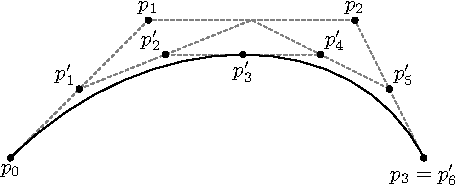
\includegraphics{subdivision}
	     \caption{A Figure}
	 \label{subd}
	\end{figure}

\clearpage %% starts a new page and stops trying to place floats such as tables and figures

\section{More Figure Stuff}
You can also scale and rotate figures.
 	\begin{figure}[h!]
	   
	       \centering
	    % DO NOT ADD A FILENAME EXTENSION TO THE GRAPHIC FILE
	    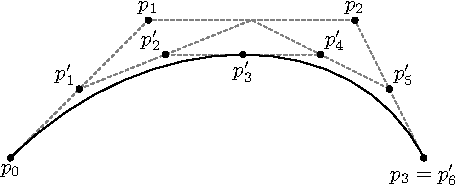
\includegraphics[scale=0.5,angle=180]{subdivision}
	    % if your figure shows up not where you want it, it may just be too big to fit. You can use the scale argument to shrink it, e.g. scale=0.85 is 85 percent of the original size. 
	     \caption{A Smaller Figure, Flipped Upside Down}
	 \label{subd2}
	\end{figure}

\section{Even More Figure Stuff}
With some clever work you can crop a figure, which is handy if (for instance) your EPS or PDF is a little graphic on a whole sheet of paper. The viewport arguments are the lower-left and upper-right coordinates for the area you want to crop.

 	\begin{figure}[h!]
	    	       \centering
	    % DO NOT ADD A FILENAME EXTENSION TO THE GRAPHIC FILE
	   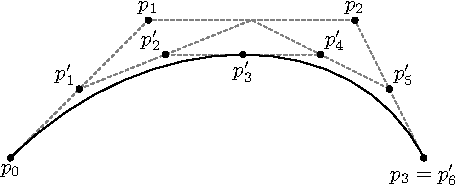
\includegraphics[clip=true, viewport=.0in .0in 1in 1in]{subdivision}
	    \caption{A Cropped Figure}
	 \label{subd3}
	\end{figure}
	
      \subsection{Common Modifications}
      The following figure features the more popular changes thesis students want to their figures. This information is also on the web at \url{web.reed.edu/cis/help/latex/graphics.html}.
           \renewcommand{\thefigure}{0.\arabic{figure}} %Renumbers the figure to the type 0.x
    \addtocounter{figure}{4} %starts the figure numbering at 4
    \begin{figure}[htbp]
    \begin{center}
   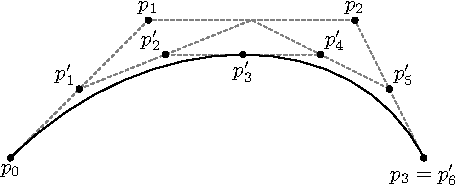
\includegraphics[scale=0.5]{subdivision}
    \caption[Flower type and percent specialization]{\footnotesize{Interaction bar plot showing the degree of specialization for each flower type.}} %the special ToC caption is in square brackets. The \footnotesize makes the figure caption smaller
    \label{barplot}
    \end{center}
    \end{figure} 

	\chapter*{Conclusion}
         \addcontentsline{toc}{chapter}{Conclusion}
	\chaptermark{Conclusion}
	\markboth{Conclusion}{Conclusion}
	\setcounter{chapter}{4}
	\setcounter{section}{0}
	
Here's a conclusion, demonstrating the use of all that manual incrementing and table of contents adding that has to happen if you use the starred form of the chapter command. The deal is, the chapter command in \LaTeX\ does a lot of things: it increments the chapter counter, it resets the section counter to zero, it puts the name of the chapter into the table of contents and the running headers, and probably some other stuff. 

So, if you remove all that stuff because you don't like it to say ``Chapter 4: Conclusion'', then you have to manually add all the things \LaTeX\ would normally do for you. Maybe someday we'll write a new chapter macro that doesn't add ``Chapter X'' to the beginning of every chapter title.

\section{More info}
And here's some other random info: the first paragraph after a chapter title or section head \emph{shouldn't be} indented, because indents are to tell the reader that you're starting a new paragraph. Since that's obvious after a chapter or section title, proper typesetting doesn't add an indent there. 


%If you feel it necessary to include an appendix, it goes here.
	\appendix

	\chapter{The First Appendix}
An appendix full of awesome
	\chapter{The Second Appendix, for Fun}
An appendix full of win


%This is where endnotes are supposed to go, if you have them.
%I have no idea how endnotes work with LaTeX.

  \backmatter % backmatter makes the index and bibliography appear properly in the t.o.c...

% if you're using bibtex, the next line forces every entry in the bibtex file to be included
% in your bibliography, regardless of whether or not you've cited it in the thesis.
  \nocite{*}

% Rename my bibliography to be called "Works Cited" and not "References" or ``Bibliography''
% \renewcommand{\bibname}{Works Cited}

%    \bibliographystyle{bsts/mla-good} % there are a variety of styles available; 
%  \bibliographystyle{plainnat}
% replace ``plainnat'' with the style of choice. You can refer to files in the bsts or APA 
% subfolder, e.g. 
 \bibliographystyle{APA/apa-good}  % or
 \bibliography{thesis}
 % Comment the above two lines and uncomment the next line to use biblatex-chicago.
 %\printbibliography[heading=bibintoc]

% Finally, an index would go here... but it is also optional.
\end{document}
